\documentclass{article}
\usepackage[utf8]{inputenc}
\usepackage{natbib}
\usepackage{graphicx}
\usepackage[utf8]{inputenc}
\usepackage{comment} % enables the use of multi-line comments (\ifx \fi) 
\usepackage{fullpage} % changes the margin
\usepackage{hyperref}
\usepackage{amsmath}
\usepackage{mathtools}
\usepackage{booktabs} % For formal tables
\usepackage{listings}
\usepackage{tabto}
\begin{document}
\noindent
\large\textbf{Software Engineering Process} \hfill \textbf{Amit Sachdeva} 

\normalsize Topic: Deliverable 1 \hfill \textbf{40084627} 

Prof. P. Kamthan \hfill Due Date: 19/July/2019

\begin{center}
    \section*{Gamma Function}
    \section*{Problem 1}
\end{center}
\section{Introduction} 
\textbf{Gamma Function: } It is commonly referred as factorial function for complex numbers. It is derived by Daniel Bernoulli. The gamma function $\gamma(z)$ is defined for all complex values of z larger than zero. Complex number can be consist of real and imaginary number, like $z = a + i b$ in which a and b can real numbers. A complex number is typically written in the form where sigma a is the real part and it is the imaginary part.
\begin{figure}[h!]
\centering
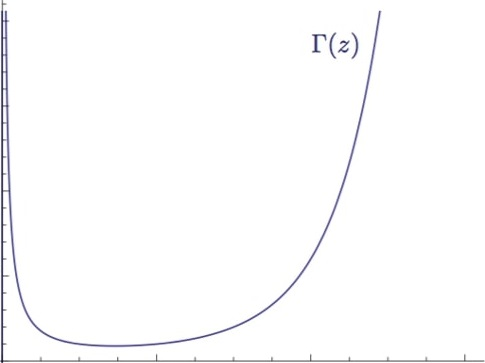
\includegraphics[scale=0.4]{gamma1}
\caption{Gamma Function}
\label{fig:Gamma Function}
\end{figure}
\section{Overall Description} 
This is a project based on gamma function in which we are making calculator for gamma value. User can insert any real value and expect real value except on boundary conditions.

\section{Stakeholders} 
\textbf{Users 1:} This function is mostly used in physics calculations. So, most important stakeholders are scientists for their calculations.
\newline \newline
\textbf{Users 2:} This function is also used in basic maths calculations or any analytically field. 



\section{Related to Function}
\subsection{Formulas}
\begin{itemize}
\item \textbf{Formula1: } $  \Gamma \left( x \right) = \int\limits_0^\infty {s^{x - 1} e^{ - s} ds} \enspace \forall \enspace Re(x)>0$
\item \textbf{Formula2: } $  \Gamma \left( 1/2 \right) = \sqrt{\pi}$
\item \textbf{Formula3: } $  n! = n*(n-1)!$
\item \textbf{Formula4: } $  \Gamma \left( x \right) = x\Gamma \left( x-1\right) $
\item \textbf{Formula5: } $  \Gamma \left( 0 \right) = undefined $
\end{itemize}
\subsection{Popular Constant Values of Function}
\begin{itemize}
\item \textbf{Constant 1: } $  \Gamma \left( 0 \right) = undefined $
\item \textbf{Constant 2: } $  \Gamma \left( 1 \right) = 1 $
\item \textbf{Constant 3: } $  \Gamma \left( 2 \right) = 1 $
\item \textbf{Constant 4: } $  \Gamma \left( 3 \right) = 6 $
\item \textbf{Constant 5: } $  \Gamma \left( 3/2 \right) = 0.886 $
\item \textbf{Constant 6: } $  \Gamma \left( -3/2 \right) = 2.36 $
\item \textbf{Constant 7: } $  \Gamma \left( -1/2 \right) = -3.54 $
\end{itemize}
\subsection{Domain of Function}
$\forall$ Real numbers excluding negative values \\
$[0, \infty)$

\subsection{Co domain of Function}
\begin{itemize}
\item It ranges from $(0, \infty)$
\item For positive integers, we returns integer value as normal factorial
\item For other real numbers, we use integral function.
\end{itemize}
\begin{center}
    \section*{Problem 2}
\end{center}
\section{Requirements/Constraints of Function}
\subsection{Requirements}
\begin{itemize}
\item \textbf{Req1}: For \textbf{Large input} in positive value, it will return infinity as \textbf{Constraint 3}.
\item \textbf{Req2}: For \textbf{negative input} $\forall x<0 $, \textbf{Function} will return \textbf{input error}, keeping in mind \textbf{Constraint 1} and \textbf{Constraint 2}
\item \textbf{Req3}: For \textbf{$x=0$}, \textbf{Function} will return \textbf{1}, keeping in mind \textbf{Constraint 1}
\item \textbf{Req4}: For \textbf{$Re(x) > 0$}, \textbf{Function} will return positive real value, keeping in mind \textbf{Constraint 1}
\end{itemize}

\subsection{Constraints}
\begin{itemize}
\item \textbf{Constraint 1}: For Input, types must be Integer, Double, Float data types
\item \textbf{Constraint 2}: We cannot \textbf{input} value of \textbf{non negative values}
\item \textbf{Constraint 3}: We cannot input the value large positive number i.e greater than 170 as it will return infinity as a programming language constraint
\end{itemize}

\begin{center}
    \section*{Problem 3}
\end{center}

\section{Algorithms}
\subsection{Pseudo Code 1}
\subsubsection{Algorithm}
This algorithm is based on calculating based on using core integral using graph like dividing whole graph in small parts and calculating each part using formula of trapezium ($ 1/2*(base1 + base2)*height $) and combining it at the end.\newline\newline
function yAxisValue(Argument x, Argument s) \{ \newline
\indent \indent Calculate the value using $value = {s^{x - 1} e^{ - s}}$\newline
\indent \indent return value\newline
end \newline
\}  \newline
 function gammaFunction(Argument x) \{ \newline
\indent \indent if x $<$ 0\newline
\indent \indent \indent \indent then raise Input Error\newline
\indent \indent if x $>$ 170\newline
\indent \indent \indent \indent then return "Infinity"\newline\newline
\indent \indent Initialize finalData with 0\newline
\indent \indent Set Interval for gap = $10 ^ {-3}$ \newline\newline
\indent \indent while loop i for range(0,Infinity)\newline
\indent \indent \indent \indent Add the finalData by using formula of trapezium using \newline 
\indent \indent \indent \indent \textbf{$1/2*gap*(yAxisValue(i) + yAxisValue(i-gap))$} \newline
\indent \indent \indent \indent increment i with gap value \newline
\indent \indent return finalData\newline
end \newline
\} \newline
\{ \newline
In main function \newline
\indent \indent Take a input of x \newline
\indent \indent Call gammaFunction with input x-1 as a argument \newline
end\newline
\}
\subsubsection{Advantages}
\begin{itemize}
\item Get More Precise Values for input as tested with existing results
\item Using basic core approach of integration
\end{itemize}
\subsubsection{Disadvantages}
\begin{itemize}
\item We are iterating the loop at a large value so it takes time
\end{itemize}
\subsection{Pseudo Code 2}
\subsubsection{Algorithm}
This algorithm is based on calculating using pre-calculated values which act as a coefficients, iterating and calculating each values using input and coefficients\newline\newline
function gammaFunction(Argument x) \{ \newline
\indent \indent if x$<$0\newline
\indent \indent \indent \indent then raise Input Error\newline
\indent \indent if x$>$170\newline
\indent \indent \indent then return "Infinity"\newline\newline
\indent \indent declare array of finalArray precalculated values\newline
\indent \indent$temp = x + constant$\newline
\indent \indent Calculate temp value using log of temp value\newline
\indent \indent declare finalValue with value 1\newline\newline
\indent \indent while loop i for range(0,length of finalArray)\newline
\indent \indent \indent \indent $finalValue += finalArray[index]/ ++temp$\newline
\indent \indent return finalValue\newline
end\newline
\}\newline
\{\newline
In main function\newline
\indent \indent Take a input of x\newline
\indent \indent Call gammaFunction with input x-1 as a argument \newline
end \newline
\}  \newline

\subsubsection{Advantages}
\begin{itemize}
\item We are using constant pre-calculated value which increase the speed of algorithm
\item This algorithm has less calculation which reduce complexity of code
\end{itemize}
\subsubsection{Disadvantages}
\begin{itemize}
\item We have generated constant value which not always give accurate value
\end{itemize}

\subsection{Final Chosen Algorithm}
\textbf{Pseudo code 1} is chosen finally for implementation over \textbf{pseudo code 2} because I am using core implementation of integration using graph which improve the accuracy of over results over using constant coefficient. Pseudo code 2 is undoubtedly fast then than pseudo code 1 but there is no much execution time difference. So overall \textbf{Pseudo code 1} is best option

\section{References}
\begin{itemize}
\item https://www.ncbi.nlm.nih.gov/pmc/articles/PMC4247832/
\item https://medium.com/cantors-paradise/the-riemann-hypothesis-explained-fa01c1f75d3f
\end{itemize}
\end{document}
